\chapter{Rio de Janeiro Mangroves} \label{ch:mangroves}

\section{\hlc[cyan]{Chapter Purpose \& Structure}}

The case study detailed in this chapter is in service to multiple objectives. First, it seeks to address Research Question 2: ``What are the sustainability benefits of collaborative development of \acp{dss} using the \acf{evdt} Modeling Framework in complex \acf{sets}?" It accomplishes this by providing a case study demonstration of Research Deliverables 2a, 2b, and 2c: 

	\begin{enumerate}[label=\emph{\alph*},itemsep=0pt,parsep=0pt]
		\item{System architecture analyses of each of the case studies} 
		\item{Development of an \ac{evdt}-based \acf{dss} for each of the case studies} 
		\item{An interview-based assessment of the development process and usefulness of each \ac{dss}} 
	\end{enumerate}
	
Through these deliverables, this chapter serves as a demonstration of the \ac{evdt} Framework. The structure of this chapter thus mirrors the components of the framework laid out in Section \ref{sec:framework}. It starts by walking through the steps of the \acf{saf} as applied to this case study in Section \ref{sec:rio-saf}. These are separated into the methodology used for each step of the \ac{saf} (Section \ref{sec:rio-saf-method}) and the results of each step (Section \ref{sec:rio-saf-results}. Then, in Section \ref{sec:rio-evdt}, it shall turn to showing relevant datasets and analysis as applied through the \acf{evdt} models. These two are separated in methodology (Section \ref{sec:rio-evdt-method}) and results (Section \ref{sec:rio-evdt-result}. These are then integrated into a prototype \ac{dss} in Section \ref{sec:rio-dss}. Finally Section \ref{sec:rio-collab} lays out how various stakeholders were collaborated with beyond the setting of requirements during the \ac{saf} process. The remaining sections examine and discuss the outcomes of this case study. The following chapter will similarly present a second case study.  

It should be noted that, as stated in Section \ref{sec:questions}, each case study also has its own objectives beyond supporting a chapter of this thesis. In this case, that means supporting policy decisions in Rio de Janeiro surrounding human wellbeing and mangrove conservation. Readers specifically interested in the socio-environmental history of the study area are pointed to Section \ref{sec:rio-context}. Those interested in environmental analyses performed in the course of this research are pointed to Sections \ref{sec:rio-evdt-e-method}, \ref{sec:rio-evdt-e-result}, and \ref{sec:rio-discussion}.

Finally, this research was begun in 2017. Field visits took place in 2019 and 2020, the latter of which was interrupted by the onset of the COVID-19 pandemic (as was this project in general). Our research and development priorities (both mine and those of our Rio de Janeiro colleagues) shifted to more urgent concerns. This means that aspects of this chapter are a couple of years old at the time of writing and various desired objectives were never reached. This is discussed further in Section \ref{sec:rio-discussion}.


\section{\hlc[green]{Systems Architecture Framework}} \label{sec:rio-saf}

The following subsections work through the six steps of the \ac{saf} originally detailed in Section \ref{sec:saf} as applied to the Rio de Janeiro mangrove case study, first as methodology and then as results. The goal is to identify what information, analyses, and other forms of decision support would be useful to stakeholders in the Guaratiba area.

\subsection{\hlc[green]{SAF Methodology}} \label{sec:rio-saf-method}

\subsubsection{\hlc[cyan]{System Context}} \label{sec:rio-context}

Rio de Janeiro has a great deal of familiarity with the descriptor \textit{iconic}. The word is frequently associated with the city's beaches, Copacabana and Ipanema, and with its festivals, such as Carnaval. So too have the city's hillside favelas found themselves as perhaps the definitive image of informal settlements and poverty in the global popular consciousness. It stands to reason that when the city hosted not just one but two megaevents in a row, the 2014 FIFA World Cup and the 2016 Summer Olympics, massive amounts of attention would be paid to the city not only by the urban planners, activists, and economists used to critiquing such endeavors, but by the international press and general public as well. As residents of distant countries, we were presented with stunning photos of the sports facilities being constructed \cite{umlaufRioCityTransformed2016} followed by equally stunning photos of their abandonment and disrepair \cite{olivaresRioOlympicVenues2017}. The academic literature is full of critiques of these events, with particular focus on the processes and effects of the major projects such as the Maracanã stadium and the Porto Maravilha redevelopment \cite{sanchezMegaeventsUrbanRegeneration2013}, as well as the displacement and responses of the directly impacted communities  \cite{talbotHumanRightsAbuses2018,viehoffPoliticsMegaeventPlanning2016}. 

This case study does not focus these stadiums and favelas. It is not, ultimately, a further elaboration on the \textit{iconic} Rio de Janeiro. Rather it seeks to examine and discuss a particular neighborhood, one that is (or rather, has been) in an out-of-the-way corner of the municipality, away from the gorgeous beaches and troubled favelas, more swamp and farm than urban, yet still important for reasons that will be made clear. This area, Guaratiba (and more specifically, the area stretching between Pedra de Guaratiba and Barra de Guaratiba), is, despite its relative remoteness in the southwestern corner of the city, still a part of Rio de Janeiro, and thus affected by the powers and forces at work in the city. To this end, after defining the study area, I will briefly lay out the relevant parts of recent Rio urban planning history, specifically the city's long fascination with grand plans and its oftentimes confusing overlay of government jurisdictions. Afterwards, we will dive into Guaratiba itself: its environment, its people, and its potential future. 

\paragraph{\hlc[cyan]{Study Area}} \leavevmode\newline

Guaratiba is a relatively rural district of Rio de Janeiro situated in the southwestern corner of the municipality. Rio de Janeiro is divided in 5 administrative zones, which are further divided into \acp{ra}, as seen in Figure \ref{fig:ras}. Guaratiba is \ac{ra} XXVI, simultaneously one of the largest of the \acp{ra} by land area and one of the smallest by population, constituting only 1.9\% of the municipal population as of 2018 with only has three official barrios (or neighborhoods) within it \cite{institutopereirapassos|datarioRegioesPlanejamentoIndicadores2018}. It is home to a mix of land uses, including decorative plant farming, multiple fishing communities, a military base and training center, a state-run biological reserve, some informal settlements, and a growing ecotourism industry. The biological reserve exists to protect the largest remaining mangrove forest within the municipality, contained primarily in the coastal region of the \ac{ra} between the Barra de Guaratiba (152 on the map) and the Pedra de Guaratiba (153). This means that the bulk of the approximately 120,000 residents of the \ac{ra} are to the north of the mangroves, but there are still approximately 20-25K people in close proximity.

These mangroves are vulnerable due to landward urbanization, including a recently opened urban transit line, and rising sea levels \cite{goldbergEcoMapDecisionsupportTool2018}. They provide a variety of ecosystem services, including serving as a mechanism for highly efficient carbon sequestration, supporting a small-scale industry of fishing and crab catching, preventing coastal erosion, and attracting the aforementioned local ecotourism industry \cite{schwenkResearchEnvironmentalSocioeconomical2008}. Government policies to conserve the mangroves can use integrated modeling tools to consider both the benefits of protecting the forests as well as the economic needs of low-income communities. This, coupled with the Rio de Janeiro municipal government's pre-existing interest in generating useful datasets and making them available online through the Data.Rio platform \cite{matheusOpenGovernmentData2014}, made the Guaratiba mangroves a particularly suitable case study for the \ac{evdt} Modeling Framework.

\begin{figure}[h]
	\centering
	\includegraphics[scale=0.5]{Figures/chap4/RA2.png}
	\caption{RAs of Rio de Janeiro. Guaratiba in blue and includes the barrios 151-153.}
	\label{fig:ras}
\end{figure}

In order to further establish the system context for the Guaratiba area, I conduct a literature review and synthesis. In particular, I use four lenses to examine the system context:

\begin{enumerate} \setlength{\itemsep}{0pt} \setlength{\parskip}{0pt}
    \item What are the broader municipal and regional dynamics impacting Guaratiba? (Section \ref{sec:rio-plans})
    \item What are the different government jurisdictions at play in the area? (Section \ref{sec:rio-jurisdictions})
    \item What is the past, current, and likely future state of the environment in Guaratiba? (Section \ref{sec:guaratiba-environment})
    \item What is the past, current, and likely future socioeconomic state of Guaratiba? (Section \ref{sec:guaratiba-people})
\end{enumerate}

\subsubsection{\hlc[yellow]{Analyze System Stakeholders}}

Our primary Local Context Experts and points of contact are at \ac{ipp}, which is the municipal data agency, and ESPAÇO, a research group at the \ac{ufrj} who study various coastal ecosystems in Brazil and elsewhere \cite{cruzClassificacaoOrientadaObjetos2007, seabraMapeamentoDinamicaCobertura2013} and who are also familiar with examining socioeconomic impacts of environmental phenomena \cite{schwenkResearchEnvironmentalSocioeconomical2008}. The latter can also be considered to be Technical Area Experts. Other Local Context Experts include a member of a local fisher association and government officials at the municipal urban development agency and the municipal environmental agency. Additional Technical Area Experts include two ecosystem services economists (one from the University of West Virginia and one from \ac{rff}) and the committee members for this thesis. The primary intended users for this case study are government officials at the \ac{ipp} who have a fair amount of experience with mapping. Future projects in this area would ideally expand that userbase to non-government individuals. 

Over the course of two field visits to Rio de Janeiro and Guaratiba, I conducted a series of interviews and meetings with various key stakeholders in the Guaratiba system, including local fishers; local academic researchers; and municipal, state, and federal government officials. I was introduced to these stakeholders using a snowball approach, starting with connections stemming from the Space Enabled Research Group and our primary point of contacts in Rio de Janeiro. Information about both contacted and noncontacted stakeholders are summarized in Table [insert].

[** insert table summary]


The interviews varied in length from 30 minutes to 1.5 hours, semi-structured, and conducted in-person. The informal meetings lasted from 30 minutes to 3 hours and were conducted in-person. With the exception of two of the interviews (noted in the table), the interviews and meetings were not recorded. For the recorded interviews, the recordings were reviewed and using to generate notes and codings. For all the others, written notes were taken during and immediately after the interview/meeting. 

[** further explain interview questions and objectives]

I coded the recordings and notes qualitatively based on the \ac{saf} in order to develop meaningful themes and conclusions, identify commonalities and differences across the stakeholders, and better understand the relationships between stakeholders. In particular, these codings were used to identify Needs, Goals, Challenges, Relationships, Functions, and Forms as discussed in the subsequent sections. 

\subsubsection{\hlc[red]{Understand Desired Outcomes \& Objectives}}

[provide details on the codings (just a paragraph or two)]


\subsubsection{\hlc[red]{Select System Functions}}

[provide detail on the function selection process (just a paragraph)]

\subsubsection{\hlc[red]{Assign Function to Forms}}

[provide detail on the form assignment process (just a paragraph)]

\subsubsection{\hlc[red]{Monitor and Evaluate Systems}}

[provide detail on the monitoring and evaluation plans (just a paragraph or two)]

\subsection{\hlc[red]{SAF Results}} \label{sec:rio-saf-results}

[add a figure summarizing the context here]

\subsubsection{\hlc[green]{System Context}}

\paragraph{\hlc[green]{Big Plans and Megaevents in Rio de Janeiro}} \label{sec:rio-plans} \leavevmode\newline

Rio has a history of being on the forefront of intentionality and long-term strategic thinking when it comes to urban planning. In 1995, it became the first city in Latin America to develop a strategic plan, something it continues to do in three-year increments to this day \cite{prefeituradacidadedoriodejaneiroPLANOESTRATEGICOCIDADE2017}. Specific programs stemming from these plans include the Favela Bairro Programme which sought to upgrade the informal settlements and the Rio-Cidade Programa which sought to revitalize certain key areas of the city \cite{aciolyc.ReviewingUrbanRevitalisation2001}.

This type of strategic planning took place alongside a broader effort in the city and across Brazil to increase democratic participation in the planning process, as the country transitioned out of a military dictatorship \cite{aciolyc.ReviewingUrbanRevitalisation2001}. This interest in blending democracy with planning could also be seen in replacement of the government-owned Municipal Computer and Planning Company with the \ac{smu} and \ac{ipp}, thereby retaining both planning and data gathering capabilities, but putting them in the hands of government offices. While Rio has never reached the same level of public participation as Porto Alegre \cite{desousasantosParticipatoryBudgetingPorto1998}, this inclination has continued to today, as seen in efforts like the Data.Rio platform, which seeks to make increasing amounts of data about the city freely available online, and the proliferation of neighborhood-level``Associação De Moradores" (Residents' Associations).

Perhaps due to its beautiful natural environment and the importance of its tourist industry (a major focus of the 1995 strategic plan), Rio de Janeiro has long acknowledged the importance of environmental conservation and sustainability when it comes to development. Even prior to 1995, the city hosted the \ac{unced}, which gave birth to the Climate Change Convention, itself the basis for international climate change agreements. Twenty years later, the city would once again play host to such a conference, this time in the form of the 2012 \ac{uncsd}, which paved the way for the creation and adoption of the \acp{sdg} by the UN General Assembly three years later. It should be made clear that Rio de Janeiro was no mere picturesque venue for these conferences. Rather, the city has taken the UN pronouncements of sustainable development seriously, publishing a Climate Change Adaptation Strategy in 2016 (utilizing entirely intra-country expertise)  \cite{prefeituradacidadedoriodejaneiroClimateChangeAdaption2016} and a Resilience Strategy in 2017 (created in partnership with the Rockefeller Foundation) \cite{100resilientcitiesResilienceStrategyCity2017}. The city is currently using a participatory process to create a Sustainable Development Plan that will detail how the city intends to contribute towards the \acp{sdg} \cite{unitednationsbrazilONUConvidaCariocas2019}.

A plethora of plans does not necessarily result in smooth sailing, however (in fact, many would say that it is directly contrary to good development \cite{easterlyWhiteManBurden2007a}). While the climate and sustainability-related plans advocate for environmental protections, energy efficiency, and waste controls, the strategic plans have focused more strongly on economic development and the tourist industry, which is related to but not identical with environmental conservation. These latter plans have explicitly espoused the use of sports megaevents (which manifested in the form of the 2014 FIFA World Cup and the 2016 Summer Olympics) as a way of attracting investment \cite{sanchezMegaeventsUrbanRegeneration2013}, a pursuit that has arguably done little to advance either sustainable development or climate change resilience, particularly as many of the recent venues were built directly on waterfront or on protected nature reserves \cite{connorsLocalGolfersTest2016}. 

Of particular relevance to Guaratiba is how the megaevent-related development reshaped transportation patterns and commercial development throughout the city. This phenomena is perhaps best explained through the use of three maps. Figure \ref{fig:relocation} shows the origin and destination of most of the favela relocation efforts (both voluntary and mandatory) in the years leading up to the World Cup and Olympics. Most of the new settlements were constructed under the \ac{mcmv} program, a federal program started in 2009 that enabled the some of the poorest households in Brazil to purchase new homes with little-to-no down payments, interest rates of near-zero, and income-adjusted monthly payments. The program was initially aimed at building one million homes nationwide, then later expanded to three million, of which more than 100,000 were assigned to the city of Rio de Janeiro \cite{nadalMinhaCasaMinha2018}. The city partly used this allocation of federal funds to support favela relocation efforts as part of megaevent-related development.

\begin{figure}[h]
	\centering
	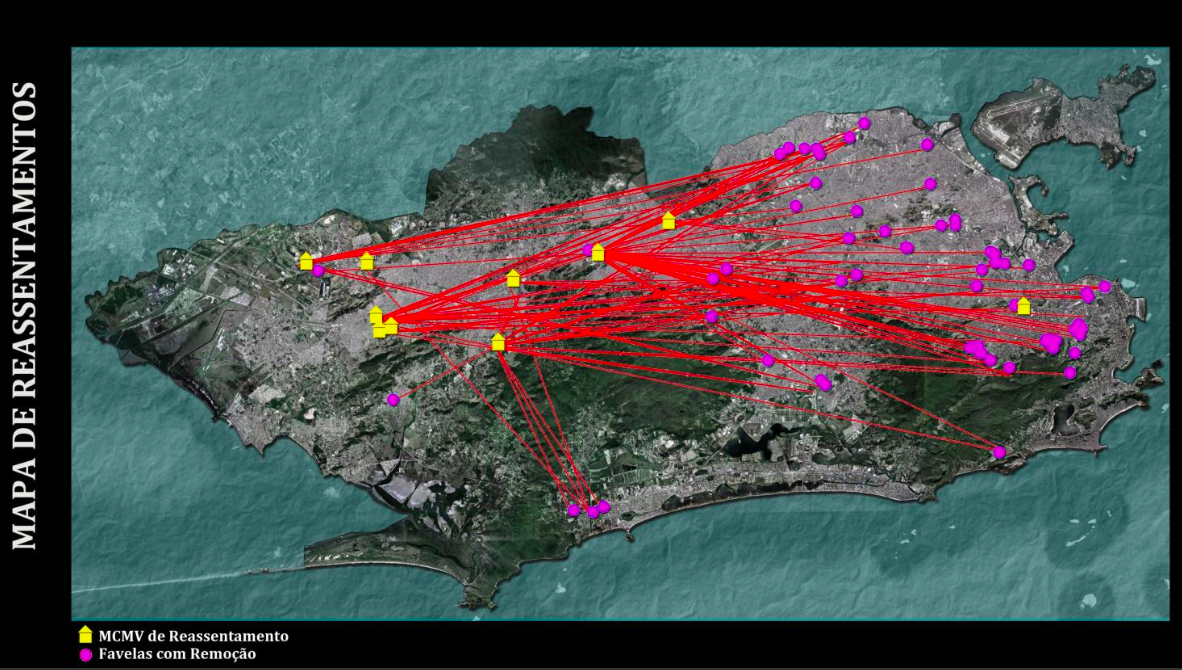
\includegraphics[scale=0.3]{Figures/chap4/Relocation.png}
	\caption[Favela Relocation Locations under MCMV between 2009 and 2013]{Favela Relocation Locations under \ac{mcmv} between 2009 and 2013. From \cite{faulhaberRioMaravilhaProjetos2012}}
	\label{fig:relocation}
\end{figure}

The relocation of favela inhabitants from east to northwest introduced problems, however. The original siting of informal settlements in Rio de Janeiro was partially driven by the availability of proximal employment. This is why historically, despite low land prices in the rural western parts of the city, most of the city's poor elected to live in high density favelas in the eastern, urban neighborhoods. Figure \ref{fig:employment} shows that while the new, formal \ac{mcmv} homes may have been higher quality than the old favela homes, they were also much further away from major centers of employment. Getting a nicer home is not much consolation for losing your job. 

\begin{figure}[h]
	\centering
	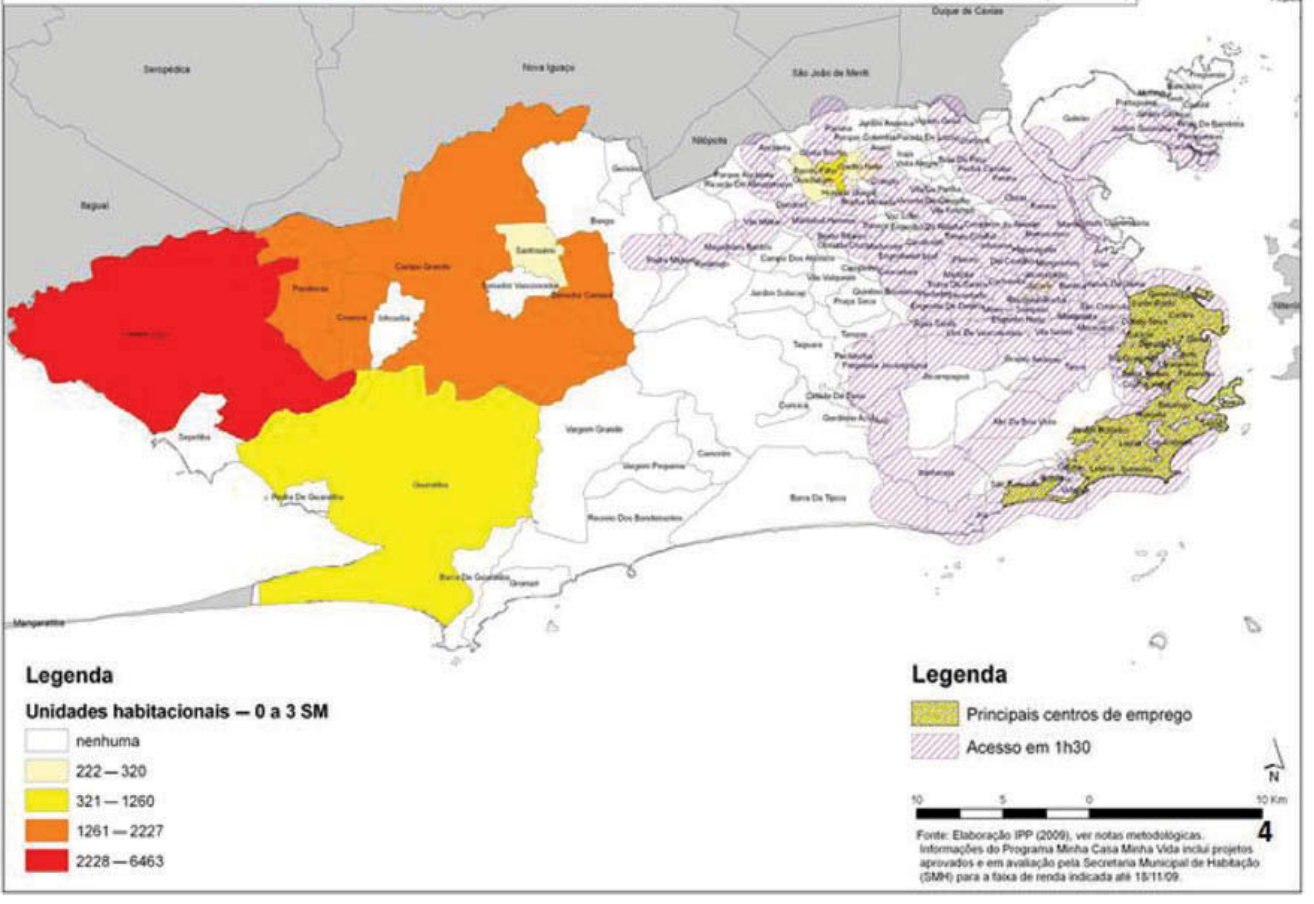
\includegraphics[scale=0.3]{Figures/chap4/Employment.png}
	\caption[Comparison of MCMV housing units and access to major employment centers.]{Comparison of MCMV housing units and access to major employment centers. From \cite{sanchezMegaeventsUrbanRegeneration2013}}
	\label{fig:employment}
\end{figure}

The Rio de Janeiro government was neither completely ignorant nor completely callous, however. As is common in the lead-up to sports megaevents, the city planned significant renovations, improvements, and extensions to the existing public transit system, as shown in Figure \ref{fig:transit}. Some of these, in particular the extension of the metro and the dedicated-lane bus Transoesto from Copacabana towards Barra Da Tijuca, were intended primarily to improve access to the major Olympic sporting venues. Many of the extensions, however were intended to better connect the northern and northwestern reaches of the city with the centers of employment, alleviating the concerns of those being relocated, while also improving accessibility for the existing residents of those areas. 

\begin{figure}[h]
	\centering
	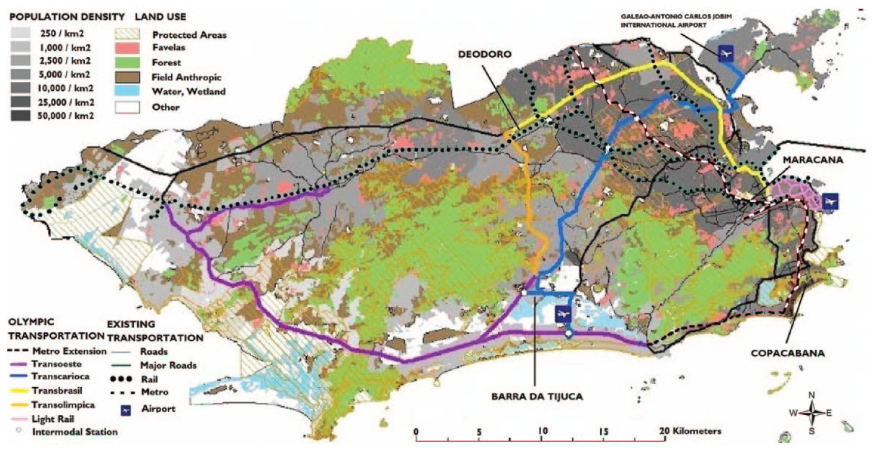
\includegraphics[scale=0.5]{Figures/chap4/Transit.png}
	\caption[Olympic-related transportation expansions and proximity to environmental protection areas]{Olympic-related transportation expansions and proximity to environmental protection areas. From \cite{kassens-noorOlympicTransportLegacies2018}}
	\label{fig:transit}
\end{figure}

Unfortunately the transit extensions were not as extensive, reliable, or high speed as initially promised \cite{wattsFuryFrustrationBrazil2014} and access to jobs for poorer communities ultimately decreased \cite{robertsonResultsAreCostly2017}. None of this directly impacted Guaratibans, however, as Guaratiba, tucked in the southwestern corner of the city, was neither the source nor destination of relocation efforts. What \textit{would} impact Guaratiba was the the Transoesto line and the related expansion of bus routes and road widths. These significantly increased the accessibility of downtown Rio de Janeiro for the largely rural Guaratibans (and vice versa). This accessibility significantly increased the value of the area for commercial activity and development, exacerbating ongoing local trends, as will be discussed further in Section \ref{sec:guaratiba-people}.

\paragraph{\hlc[green]{Overlapping Jurisdictions in Guaratiba}} \label{sec:rio-jurisdictions} \leavevmode\newline

While the city of Rio de Janeiro has busied itself with high-level plans, the municipal government is by no means the only government player in the city. Brazil has a whole has significant amounts of jurisdictional overlap between its municipal, state, and federal levels of government, when compared to countries such as the United States \cite{coutoImitationCoercionState2018}. This is particularly true for the city of Rio de Janeiro, which for more than 200 years until 1960, was the capital of Brazil. To this day, numerous institutions and roles within the city that elsewhere would be managed by the state or municipal governments are still federally administered. For example, there are numerous individual public schools, from primary through tertiary, that are run by either the city, state, or federal government, fairly independently of one another. In the field of environmental management, both the federal and state constitutions have chapters on the environment, and the municipality has its own an environmental secretariat. These distinct sources of authority are often visible in regulatory law, such as the separate endangered species lists maintained by the federal \cite{institutochicomendesdeconservacaodabiodiversidadeListaNacionalOficial2014} and state governments \cite{institutoestadualdoambienteListaEspeciesFauna}.

The most relevant aspect of these overlapping environmental jurisdictions when it comes to the Guaratiba area is the Carioca Mosaic\footnote{``Cariocan" is the demonym for inhabitants of Rio de Janeiro and ``Carioca" or ``Carioco" is an often-used adjectival form.}. This term refers to the federally-coordinated collection of federal, state, and municipal environmental conservation areas in the greater area of the city of Rio de Janeiro \cite{teixeiraPORTARIANo2452011}. Within the Mosaic, the federal government's \ac{icmbio} administers one national park and one national monument; the state government's \ac{inea} administers one state park, two environmental protection areas, and one biological reserve; and the municipal government's \ac{smac} administers 14 nature parks, two environmental protection areas, and a natural monument.

Of these various units, the following are in or in direct proximity to the Guaratiba area:

{\setstretch{1.0}
\begin{itemize}
	\item \ac{apa} Ambiental das Brisas (municipal)
	\item \ac{apa} da Orla da Baia de Sepetiba (municipal) 
	\item Parque Natural Municipal da Serra da Capoeira Grande (municipal)
	\item Parque Nacional Municipal da Prainha (municipal)
	\item Parque Nacional Municipal de Grumari (municipal)
	\item \ac{rbag}\footnote{Until 2006, this land was controlled by the nearby Brazilian Army \ac{ctex}, which continues to occupy a significant amount of land in the Guaratiba area and maintains some facilities within the \ac{rbag}. Similarly to other military administered lands in various parts of the world, \ac{ctex}'s control of this land results in a kind of quasi-environmental protection that is simultaneously less formally determined than actual environmental conservation areas but much more stringently enforced in practice. For example, there is an army vehicle workshop that disposes of waste directly into the mangroves, but commercial activities and unauthorized human access are strictly forbidden \cite{herzogGuaratibaVerdeSubsidios2009}.} (state)
	\item \ac{apa} Sepetiba II (state)
	\item Parque Estadual da Pedra Branca (state)
\end{itemize}}

This means that those who live and work in the Guaratiba area will regularly come into contact with eight different municipal and state-run conservation areas that are then collectively coordinated by the federal government. Such an arrangement has both benefits and costs. On the positive side, it can help ensure a certain minimum level of environmental protection amid shifting government priorities. For instance, at the time of writing, the state government of Rio de Janeiro is prioritizing security \cite{kaiserRioGovernorConfirms2019} while the federal government is actively scaling back environmental protections \cite{simoesBrazilBolsonaroEnvironment2019}. If one of these levels of government were solely in charge of environmental protection within the city of Rio de Janeiro, significant harm to the environment might occur, but since there are overlapping jurisdictions, the municipal government can continue to guarantee some minimum level of protections. Unfortunately, this system can (and does) not only lead to perhaps overly cumbersome permitting requirements for certain development projects, but can also lead to a diffusion of responsibility for environmental protections and inconsistent enforcement. 
 
This confusion of jurisdiction can have real consequences for residents of the area, particularly the disenfranchised. Take the case of Araçatiba, a small favela almost completely surrounded by the \ac{rbag}. The favela ended up in its current position in the 1970s after commercial development (specifically television filming) pushed residents away from their previous location. At the time, this land was controlled by the Brazilian Army \ac{ctex}. In 2006, the \ac{ctex} transferred most of the land in this area to the state government to form the \ac{rbag} and to protect the local mangrove forests. Some additional land, including the Araçatiba favela, was transferred to the civilian federal government. Over the next several years, the federal government took various measures to formalize the settlement, only to reverse course in 2014 and seek evictions instead \cite{chisholmWhoInvadingWhom2017}. The mayor at the time, Eduardo Paes, promised to prevent these evictions, but his successor did not follow suit, resulting in the demolition of several homes in 2017 and the threat of continued demolitions in the months to come \cite{stroblSOSAracatibaCommunity2018}. After protests organized by the favela residents, the federal government and \ac{inea} (the state environmental agency) apologized for the demolitions. Meanwhile, progress towards formal titling has stalled as it is dependent on homes being ``upgraded," which the city government has shown little interest in pursuing. Amid all of this is a somewhat bizarre digression that the federal government claimed that proper notice had been given prior to the demolitions via a message delivered to the president of the Araçatiba Residents Association, an organization that had not met in more than ten years \cite{stroblFourCoreCriticisms2018}. 

To summarize, the federal government tore down homes on federal land after being prevented for several years from doing so by the city government. The ensuing protests resulted in an apology by the state government and a refusal by the city government to certify the formalization of the settlement, which is still on federal land.

Of course, one favela is not necessarily representative of an entire region. The next two chapters will thus explore how the themes of this section and the previous section impact the people and environment of Guaratiba.

\paragraph{\hlc[cyan]{The Environment of Guaratiba}} \leavevmode\newline \label{sec:guaratiba-environment}

The distinguishing environmental aspect of the coastal Guaratiba area is its significant mangrove forest, made of five different mangrove species. Prior to colonization, most of the Rio de Janeiro coastal areas were either mountains or covered by mangroves. Over the centuries, the lowland mangrove forests were incrementally destroyed and filled in order to accommodate the growing city. The remaining mangrove trees of the greater Rio area, shown in Figure \ref{fig:mangrove-extent}\footnote{The methodology used to generate this and other original figures in the section are presented in Section \ref{sec:rio-evdt-e-method}.}, are confined primarily to northern Guanabara Bay (outside of the municipality) and eastern Sepetiba Bay (the bay on the western side of the city). This means that the Guaratiba forest, and the \ac{rbag} in particular, is the largest copse of mangroves within the city’s jurisdiction. These mangroves provide a variety of ecosystem services, including serving as a mechanism for highly efficient carbon sequestration, supporting a subsistence industry of fishing and crab catching (supporting vulnerable, juvenile shrimp in particular \cite{costaPensarMarPara1992}), preventing coastal erosion, and attracting a local ecotourism industry. Even these trees are under an ongoing threat.

\begin{figure}[h]
	\centering
	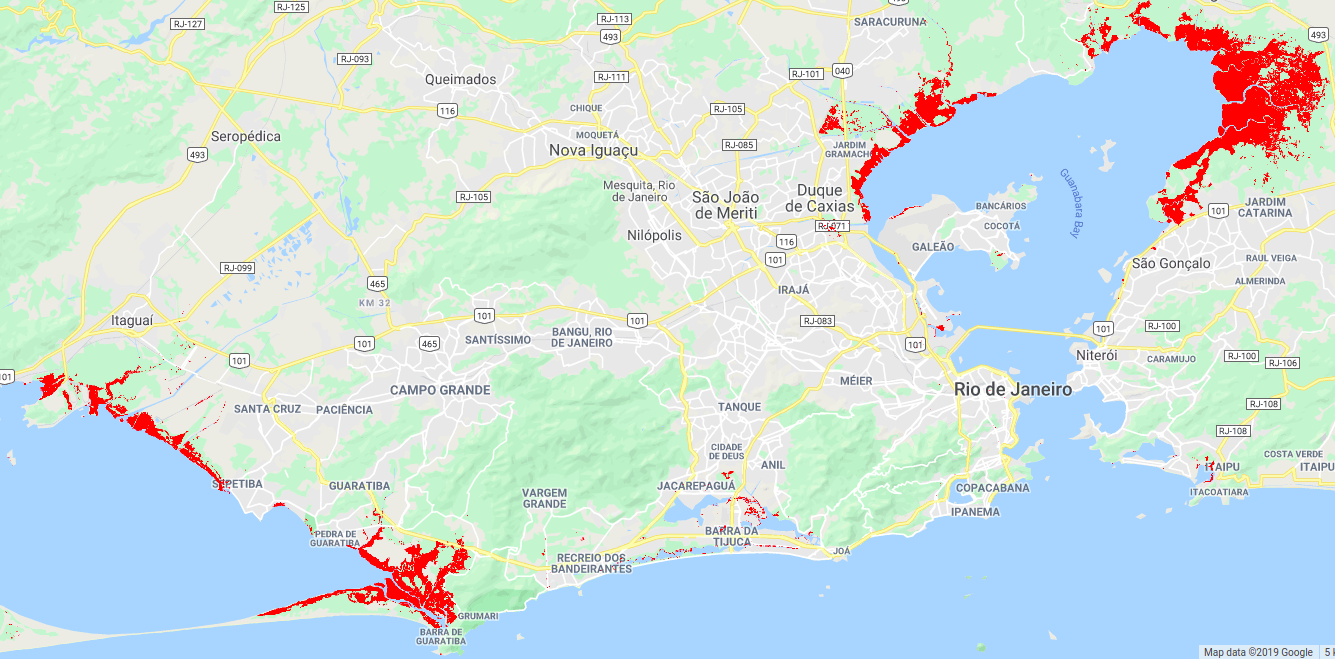
\includegraphics[scale=0.25]{Figures/chap4/MangroveExtent.png}
	\caption[Mangrove extent in the greater Rio de Janeiro area in 2018]{Mangrove extent in the greater Rio de Janeiro area in 2018, as estimated using a combination of Landsat, Sentinel, and PALSAR imagery.}
	\label{fig:mangrove-extent}
\end{figure}

Just up the cost from Pedra de Guaratiba, in the Santa Cruz \ac{ra}, the Ternium steel mill opened in 2010\footnote{Ternium purchased the steel mill in 2017. At its opening in 2010, the factory and associated port were operated by Thyssenküpp.}. This mill, along with its associated facilities, including an expanded canal, a bridge, a dam, and dredging of the bay directly replaced or caused the death of a significant number of mangroves (approximately 145 hectares) \cite{ecologusESTUDOIMPACTOAMBIENTALE2005}. Various indirect damages, including pollutants, silt disturbances, and changes in hydrology have resulted in further loses over the past several years \cite{lopesTerritorialidadesEmConflitos2013}. These effects are visible in the northwest corner of Figure \ref{fig:mangrove-ndvi-anomaly}. In this figure, red indicates damage to mangroves, including both decay and outright losses. Green indicates growth, both of existing trees and of new trees.

\begin{figure}[h]
	\centering
	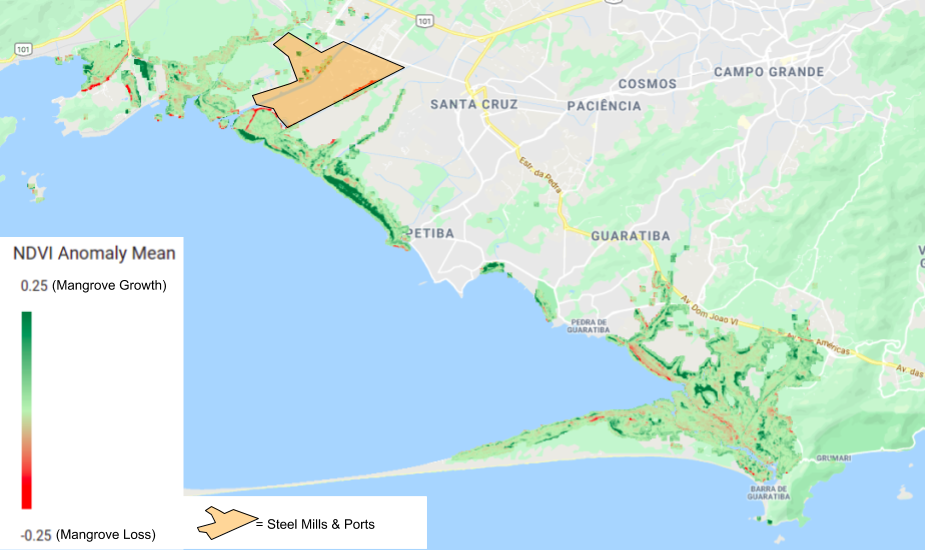
\includegraphics[scale=0.4]{Figures/chap4/NDVIanomaly_v2.png}
	\caption[Change in Guaratiba area mangrove health from 2000 to 2018]{Change in Guaratiba area mangrove health from 2000 to 2018, with the Gerdau Cosigua and Ternium steel mills indicated.}
	\label{fig:mangrove-ndvi-anomaly}
\end{figure}

While outside our direct area of interest, the steel mills of Santa Cruz have indirect effects on Guaratiba and are demonstrative of the results of potential industrial development further down the coast. In Guaratiba proper, the direct human-interfaces with the \ac{rbag} include \ac{ctex} in the center of the reserve, the Barra de Guaratiba neighborhood to the southeast, the Ilha de Guaratiba neighborhood\footnote{Ilha de Guaratiba is technically just a subdivision of Barra de Guaratiba. That said the two names are typically used to refer to different areas that have substantially different histories and economies and are only connected by a strip of land. Barra de Guaratiba is the urban cluster on the coast at the southern tip of the \ac{ra}. It was historically a fishing village and more recently a tourist destination. Ilha de Guaratiba, on the northern end of the official neighborhood along the highway, is a historical agricultural marketplace. The use of these names in this paper will stick to the common usage, particularly as we are more interested in the coastal regions rather than more inland areas such as Ilha de Guaratiba.} to the northeast, the Embrapa Agroindústria de Alimentos to the north, and the Araçatiba favela on the northeastern edge. Most of these areas are clearly visible in Figure \ref{fig:rbag}.

\begin{figure}[h]
	\centering
	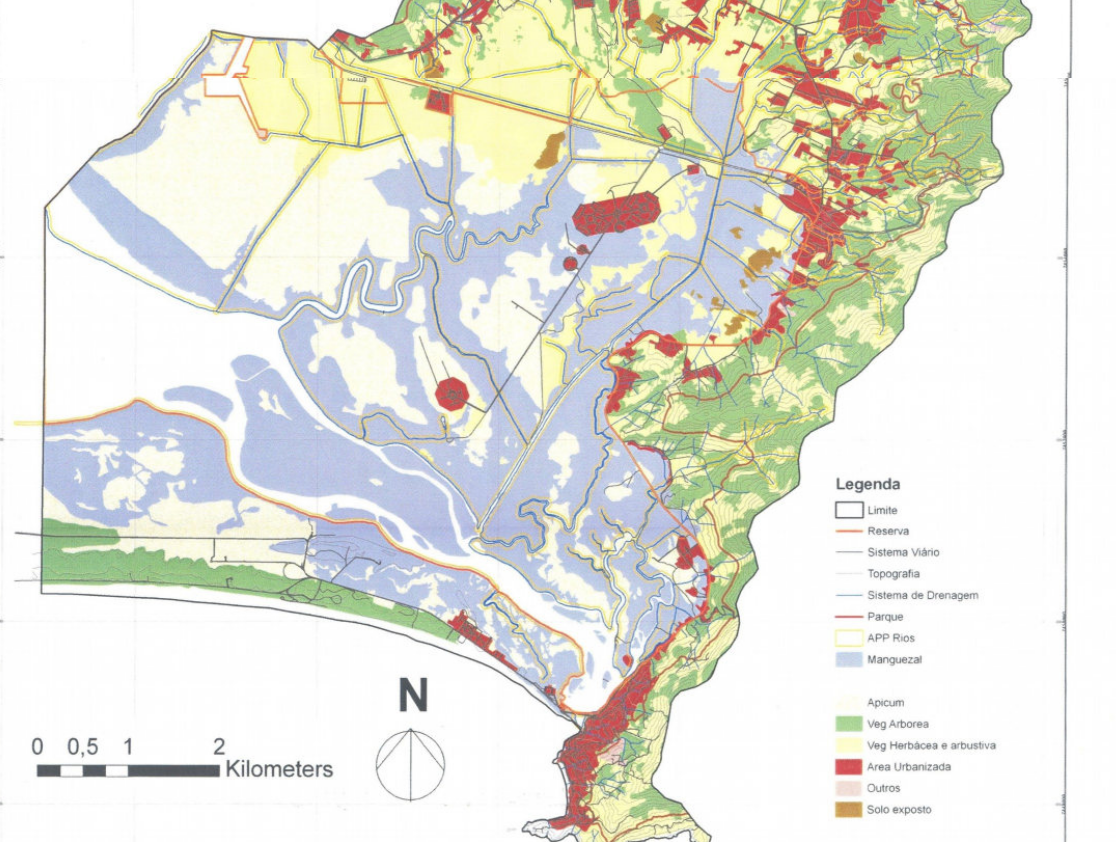
\includegraphics[scale=0.3]{Figures/chap4/RBAG.png}
	\caption[Map of RBAG and nearby urbanization]{Map of RBAG and nearby urbanization. Excerpted from \cite{herzogGuaratibaVerdeSubsidios2009} and originally made by IPP.}
	\label{fig:rbag}
\end{figure}

The health of the \ac{rbag} mangroves is a mixed bag. There has been some damage to certain sections of the forest, partly due to an invasive insect species and partly due to the increased sewage flows created by an increasing population and increased commercial activity. The dumping of waste in informal landfills, even when outside the mangrove forest itself, can still cause damage, as flows of water can be diverted or blocked, killing off sections of mangroves \cite{castroOSDESAFIOSPLANEJAMENTO2012}. All of this is driven by the fact that while there are significant legal environmental protections within \ac{rbag}, there are essentially no restrictions on development and activity just outside of the reserve, despite the fact that the mangrove forest occupies one of the primary outlets of regional drainage basin.

One component of the mangrove forest that is most directly threatened by commercial development are not the mangroves themselves, but the \textit{apicun}, hyper-saline mudflats created by the mangroves in various places on the interior and edge of the forest. These flats provide a variety of important ecological functions, such as serving as migratory stops and breeding grounds for thirty-nine species of birds\footnote{It is perhaps worth mentioning that this number used to be higher. For instance, Guaratiba takes its name for the local word for the scarlet ibis bird: \textit{guarás}. This bird is no longer found in the Rio de Janeiro area, pushed out due to a declining availability of its preferred habitat, the mangroves.} and homes for twelve species of crabs (a major target of local fishers) \cite{vicenteAvaliacaoHidrogeologicaRegioes2010}. They also represent a of land that the mangroves spread into when pressured from other directions. Despite these important functions, the apicuns are not as well protected as the mangroves themselves under the law and are commonly viewed by the public as wasted land that serves no purpose and thus ripe for development.

Additionally, part of the aforementioned transit expansion efforts was the construction of the first highway through the region, Av. D. João VI. This highways has isolated a section of mangrove forest from the main \ac{rbag} with implications that are yet to be seen. One key consequence of the highway is that the mangroves no longer have a mechanism for moving inland in the face of seaward pressures, such as a rising sea level that may take place over the coming decades.

\paragraph{\hlc[green]{The People of Guaratiba}} \label{sec:guaratiba-people} \leavevmode\newline

Guaratiba has historically had such a small population largely been due to its relative isolation. Separated by mountains on the east from the primary urban core and on the north from the more heavily populated Campo Grande \ac{ra}, Guaratiba is largely rural and heavily forested. Since the decline of colonial-era plantation farming, the residents have primarily engaged in subsistence and near-subsistence commercial activities, including artisanal fishing, farming, and ranching (including of frogs). The products of this economic activity were typically sold (via local distributors) in outdoor markets (called \textit{fieras}) throughout the Rio de Janeiro city. This largely informal supply chain kept residents somewhat isolated from the globalized agricultural markets that drove industrial farming in other parts of the city \cite{fernandesDecodificandoGeografiasPreteritas2010}.

By most development metrics, the inhabitants are some of the worst off in Rio de Janeiro, with low rates of education, more children per family, and poor health. An example of the latter can be found in the fact that approximately a quarter of the dogs in the area carry \ac{avl}, a typically fatal parasite, and human cases are relatively common, particularly in the Barra de Guaratiba area, despite control efforts \cite{cabreraCanineVisceralLeishmaniasis2003}. Over the past few decades, however, the the area has been experiencing rapid growth recently, significantly outpacing the city as a whole \cite{pizzolatoLOCALIZACAOESCOLASPUBLICAS2013}. Much of this was driven by increasing industrial employment opportunities in Campo Grande and Santa Cruz, to the north, of which the aforementioned steel mills are just one example. These areas have historically been significantly easier to reach than the core of Rio de Janeiro to the east. The more recent transit expansion projects have accelerated this trend, enabling easier access to Campo Grande and Santa Cruz. The improved connections eastward have also allowed for a more substantial ecotourism industry focused on the coastal mangrove forests and for a more substantial regional tourism (i.e. tourists from other parts or Rio de Janeiro) spending the weekends at the beaches of the area. These latter tourists have also begun purchasing second homes (vacation homes) in the area, particularly in Barra de Guaratiba, driving commercial development of condominiums and restaurants \cite{herzogGuaratibaVerdeSubsidios2009}. Such condominiums first entered the Guaratiba \ac{ra} in the 1990s and have spread to Barra de Guaratiba in the past 15 years, as transportation infrastructure to the peninsula has improved \cite{fernandesDecodificandoGeografiasPreteritas2010}. 

Such growth has itself introduced certain additional problems. The area was already characterized by low levels of education (4.7 years of school on average, by some estimates), and the increased population seems likely to overwhelm the existing school system, an issue further complicated by the fact that, due to the rural nature of the region, many students are already more than three kilometers from the nearest school and thus cannot easily be reassigned to further, emptier schools. One analysis of the \ac{ra} estimated a deficit of nearly 35,000 seats by 2020, despite low rates of attendance \cite{pizzolatoLOCALIZACAOESCOLASPUBLICAS2013}. One issue is that there are few mechanisms for community organization in the area. As mentioned earlier, Araçatiba did have a Residents Association, only for it to dissolve more than ten years ago. Now they find themselves trying to work with a city-wide Conselho Popular to effectively advocate for themselves \cite{stroblFourCoreCriticisms2018}. Even the more formal neighborhoods of Guaratiba typically have either ineffectual or nonexistent associations \cite{herzogGuaratibaVerdeSubsidios2009}. On the economic rather than residential side, frog ranchers are virtually solitary \cite{borinUMAABORDAGEMASSOCIATIVISMO2013}, as are many of the farmers. Perhaps the primary organized group in the area are the artisanal fisherman, who participate in a variety of local and regional associations of varying degrees of formality \cite{lopesTerritorialidadesEmConflitos2013}.

The continued commercial and industrial development threatens to displace many of the historical communities of Guaratiba. In the 1970s, Araçatiba was created after informal settlements were forced to move by a film studio. More recently, the opening of the Ternium steel mill, in addition to its environmental impacts discussed earlier, effectively excluded artisanal fishing activities in a significant portion of the Sepetiba Bay. While the effects of this are more directly born by neighboring Sepetiba, fishers from that area have been forced eastwards, thereby impacting Guaratiba fisherman, particularly the approximately 1,000 fishers who reside in Pedra de Guaratiba \cite{lopesTerritorialidadesEmConflitos2013}. These fishers are also pressured due to technological adoption by the more large-scale, commercial fishers. The increasing prevalence of industrial trawl fishing over the past few decades in the Sepetiba Bay (instead of more targeted, historical fishing methods), has resulted in the increased catching of juvenile and unintended fauna, as well as stirring up the silt on the bottom of the bay. This has led to increased tensions and conflicts between the the industrial and artisanal fishers \cite{begossiMappingSpotsFishing2001}, somewhat attenuated by the (illegal) ability of the artisanal fishers to operate inside the mangrove forests. This ability is by no means guaranteed, however. Fishing is nominally prohibited within the \ac{rbag}. This prohibition is currently rather poorly enforced, as part of a more board set of allowances provided to local (typically informal) residents. Another example of this allowance is that the bounds of the \ac{rbag} have, during each update, been intentionally drawn to exclude existing settlements \cite{castroOSDESAFIOSPLANEJAMENTO2012}. That said, a future policy change could result stricter enforcement and in yet further encroachment on locals’ means of subsistence. 

As Guaratiba has become more connected to the rest of the city and commercial interests have increasingly moved in, small-scale farmers have been negatively impacted as well as the fishers. The open-air fieras have been increasingly replaced by supermarkets, depriving the farmers of a means of selling their produce. Many of the farmers adapted by switching from food produce to ornamental plants, something that Guaratiba has developed a reputation for over the past several decades \cite{fernandesDecodificandoGeografiasPreteritas2010}. 

All of this is to say that isolated, rural, and poor Guaratiba be none of these things before too long. But will the Guaratibans benefit or merely be replaced? And what will happen to the natural environment that has supported them for so many generations?

Perhaps the primary conclusion of this high-level examination is that both the people and the environment of coastal Guaratiba are under active threat from a multitude of directions. Local environmentalists have a saying about this: “Guanabara is the past, Guaratiba is the present, Paraty is the future.” By this they mean that Guanabara Bay, which downtown Rio de Janeiro sits upon, is a lost environmental cause. Paraty, an area approximately 230km to the west of Rio de Janeiro, is relatively well preserved and unlikely to face serious human pressures in the next few decades. Guaratiba is where the current fight is. 

But while those who use this phrase are typically referring solely to the environment, it seems to be true for the people of Guaratiba as well. And the city, caught up in its grand Rio-wide plans for cleaning up the east and developing the north, seems not to have realized this. As one community leader recounted about an interaction with the mayor in 2018: ``The mayor looked at me and asked, `Where is Araçatiba? I don’t know.’ I said, `By Barra da Guaratiba.’ And he said, `Where is Barra da Guaratiba?'" \cite{stroblFollowingRecentEviction2018} Up until now, to the extent that the environment, and the mangrove forests in particular, have been protected, it has not been through government protection, but rather due to isolation and benign neglect. While the local residents have by no means led zero-impact lives, they at least had direct economic incentive in the preservation of the flora and fauna of their region. This is not true of the industrial and commercial development rapidly occurring the region.

Analysis and reports have already been commissioned on a variety of specific topics in the area, from reforming the educational system of Guaratiba \cite{pizzolatoLOCALIZACAOESCOLASPUBLICAS2013} to the installation of green infrastructure \cite{herzogGuaratibaVerdeSubsidios2009} to means of protecting both the marine life and the artisan fishers of the area \cite{lopesTerritorialidadesEmConflitos2013}. A comparison of such reports does bring to light certain key themes, some high priority action items that the city or region could pursue. These include:

\begin{itemize}[itemsep=0pt,parsep=0pt]
	\item{Create a proper sewage and water treatment system. This would improve the health of both the people and the environment and could make use of the natural drainage geography of the Guaratiba basin.}
	\item{Create a tiered licensing authority to permit certain low-impact artisanal activities in protected areas, while maintaining restrictions on higher impact activities. Once again, this helps the environment while also providing some degree of economic security for the historical residents.}
	\item{Strengthen environmental protections in forest-adjacent areas, such as construction limits in the Barra de Guaratiba neighborhood. This would prevent indirect pressures on the mangroves and slow both real estate speculation and commercial development, thereby preventing existing residents from being forced out. }
\end{itemize}

These items are merely specific, ad hoc solutions to a broader, meta-problem. Despite the overabundance of municipal, state, and federal government agencies operating in the area, there is no cohesive governance of the environment, the local residents (largely informal settlers), and their interactions. Without this, it is unlikely the any of these ideas will be properly implemented and broader economic forces healthily channeled. There are multiple options for such a governance structure. It could be a top-down entity, one that manages the entire drainage basin, such as the Tennessee Valley Authority or any of its numerous imitators around the world. It could also be a bottoms-up, mass participatory effort by the various communities of the area. Either way, such an entity would be able to not only implement these high priority items, but a host of others as well, such as managing the currently ad hoc diverting of the numerous regional waterways by government agencies, companies, and individuals, much to the detriment of the people and mangroves living downstream.

Unfortunately, neither option seems particularly likely at this time. As mentioned earlier, the city, state, and federal governments are either focused on other things or actively inamicable to such an effort. The residents, for the most part, have no tradition of collective action. Many residents have complained that, despite the relatively abundant land, there are essentially no public spaces in these communities \cite{herzogGuaratibaVerdeSubsidios2009}. They (rightly) decry an inattentive municipal government, but also take no action to create such spaces themselves or effectively agitate for their creation. 

The author does not have the expertise or the experience with the region necessary to either recommend a specific course of action or predict the likely outcome these ongoing changes in Guaratiba. What can be said with certainty is that there is a real need for awareness raising in the area. Much of the data discussed in the past few sections and contained in most of the references, is qualitative and anecdotal. While hard facts and demonstrable harms are no substitute for an engaged populace or an interested government, they can be a first step towards creating such things. The remainder of this chapter will be aimed at this topic.

\subsubsection{\hlc[yellow]{Analyze System Stakeholders}}

[add more discussions of who the stakeholders are]

[revisit and update stakeholder map below]

\begin{figure}[h]
	\centering
	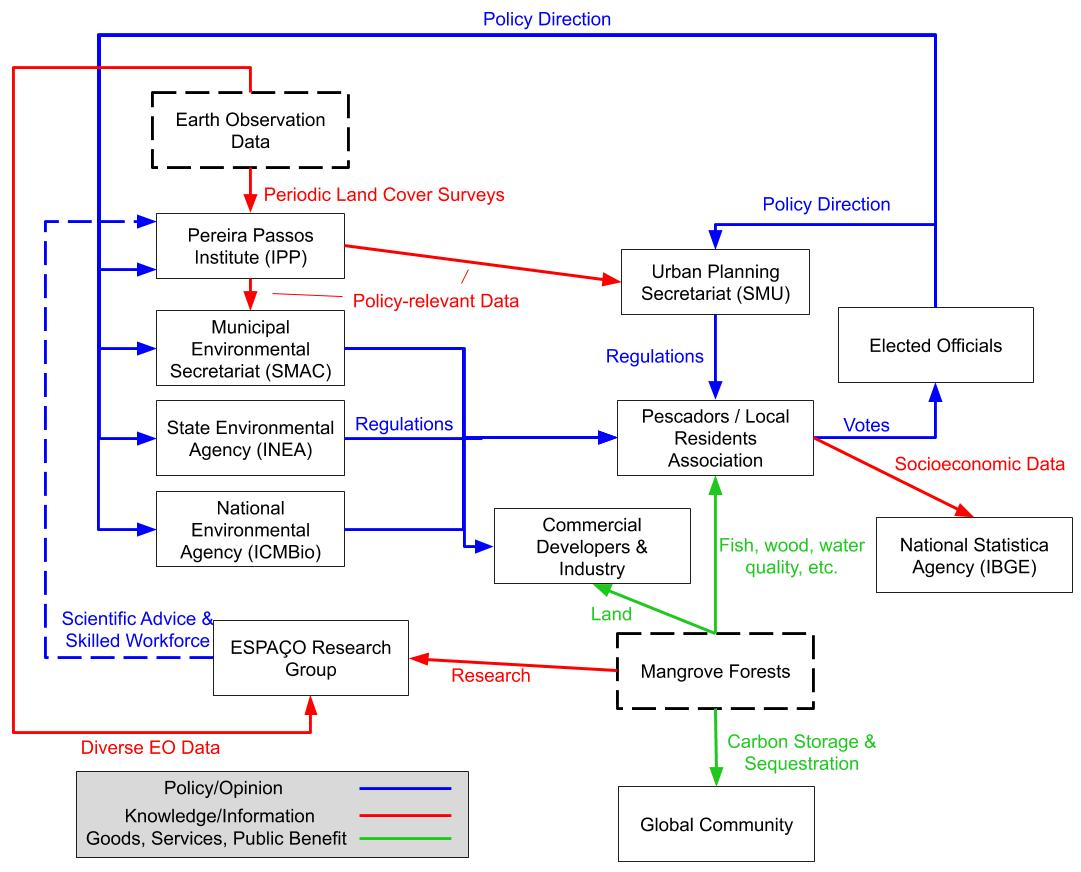
\includegraphics[scale=0.3]{Figures/chap4/Stakeholder_Map_v2.jpg}
	\caption[Stakeholder Map for the Mangrove Forests of Rio de Janeiro]{Stakeholder Map for the Mangrove Forests of Rio de Janeiro}
	\label{fig:rio_stakemap}
\end{figure}

\subsubsection{\hlc[red]{Understand Desired Outcomes \& Objectives}}

[walk through the summary of stakeholder needs outcomes, and objectives, as identified from the interviews; can refer back to Section \ref{sec:saf}]

[add table summarizing needs, outcomes, objectives]

\subsubsection{\hlc[red]{Select System Functions}}

[explain the primary questions to be answered by the EVDT analyses and the DSS]


\subsubsection{\hlc[red]{Assign Function to Forms}}

[explain the general DSS concept chosen]

\subsubsection{\hlc[red]{Monitor and Evaluate Systems}}

[discuss time scale and covid interruption]

[discuss evolving situation, desired outcomes]

\section{\hlc[cyan]{EVDT Application}} \label{sec:rio-evdt}

The following subsections walk through the components of the system from an \acf{evdt} perspective, detailing what models were used and the results of those models. Before proceeding though, it is worth stating what exactly each of the four components of \ac{evdt} mean for this system. Returning to the four questions from Section \ref{sec:evdt-questions}, we ask the following:

\begin{enumerate}[itemsep=0pt,parsep=0pt]
	\item \textbf{What is happening in the natural environment?} What are the impacts of seal-level rise and urban expansion on the mangrove forests? What role do complex secondary factors such as sedimentation change due to land use conversion and organic discharge due to agricultural activities, play in determining mangrove growth? 
	\item \textbf{How will humans be impacted by what is happening in the natural environment?} What impact do the designation of natural reserves have on the community? What effects would the lack of mangroves have on the city? What is the value of the carbon sink of mangrove forests?
	\item \textbf{What decisions are humans making in response to environmental factors and why?} How are planning policies such as restricted land use conversion in certain protected natural reserves developed? How are other centralized and decentralized decisions made, such as the rate of urban expansion or the development of transportation infrastructure? 
	\item \textbf{What technology system can be designed to provide high quality information that supports human decision making?} What satellite, aerial, and in-situ sensing platforms are needed by the municipality to accomplish their mission?
\end{enumerate}

% [**consider adapting this text for here or elsewhere in this chapter]]

%The mangrove forest is a special type of forest which grows in between land and sea. They have many important ecological and environmental properties, such as stabilizing the shorelines \cite{gedan2011present} and providing a habitat for a wide range of species \cite{ronnback1999ecological}. Although the total area of mangrove forests is not significant, their significance in maintaining a healthy coastal ecosystem is fundamental.
%
%In Rio de Janeiro, mangrove forests in Planning Area 5 are highly vulnerable due to both landward urbanization pressure, including a recently opened urban transit line, and seaward pressure from rising sea levels. Therefore, a model to evaluate both environmental risks, such as rising sea levels, and social risks, such as land use conversion into urban or agricultural use, is needed to holistically understand questions related to the protection of mangrove forests in Rio de Janeiro.

%An integrated model is the only way to capture the wide variety of biological behaviors of mangrove forests that can occur in response to certain environmental changes. For instance, mangrove's response to rising sea levels depends on sedimentation level in shoreline areas\cite{gilmanThreatsMangrovesClimate2008}, which can be altered due to human activities such as residential development \cite{lacerdaluizandmenezesmarceloandmussimolisanimauricioChangesMangroveExtension2007}. Mangrove forests have a viviparous reproduction system with seeds that are buoyant and can remain dormant until being transported to a suitable environment by the waterways \cite{sussexGrowthMetabolismEmbryo1975}. Therefore, the logic map underlying the integrated model must incorporate both the primary and the secondary factors linking together environmental and social factors. By capturing these linkages, the growth of mangrove forests can be simulated for scenarios that differ on a variety of factors, including the rate of mangrove reproduction, the sea level rise rate, and preference for proximity to transportation in residential and agricultural development.
%
%Additionally, an integrated model could help evaluate current urban planning policies in Rio de Janeiro. Currently several regions within the natural reserve, i.e. a subset of total mangrove forests, are protected against any land use conversion. With such a model, new boundaries could be considered and other potential policies could be investigated, such as various urban expansion rates, various transportation infrastructure scenarios, and more sophisticated restriction policies on land use conversion.

With these questions and goals in mind, a specific instance of the integrated model framework can be represented as shown in Figure \ref{fig:rio-evdt-flow}. In order to develop such a model, a number of steps remain to be completed. Some of the most notable include:

\begin{itemize}[itemsep=0pt,parsep=0pt]
    \item Determination of certain parameters based on historical data. These include the rate of sea level rise and the rate of urban and agricultural expansion, both of which should be identifiable from a combination of satellite data and local in-situ measurements.
    \item Collection of various demographic and social data to improve risk estimation methods for the impact of the loss of mangroves. These include population data, urban land use types, and their differential impacts on local forests. For instance, some evidence suggests that particular residential land use types, such as favelas, may lead to more severe deforestation impacts \cite{herzogLocalAssessmentRio2013}.
    \item Better understanding of the civic decision making process in Rio de Janeiro. This is necessary in order to identify what urban development policies should be simulated using the integrated model.
\end{itemize}


\begin{figure}[H]
\centering
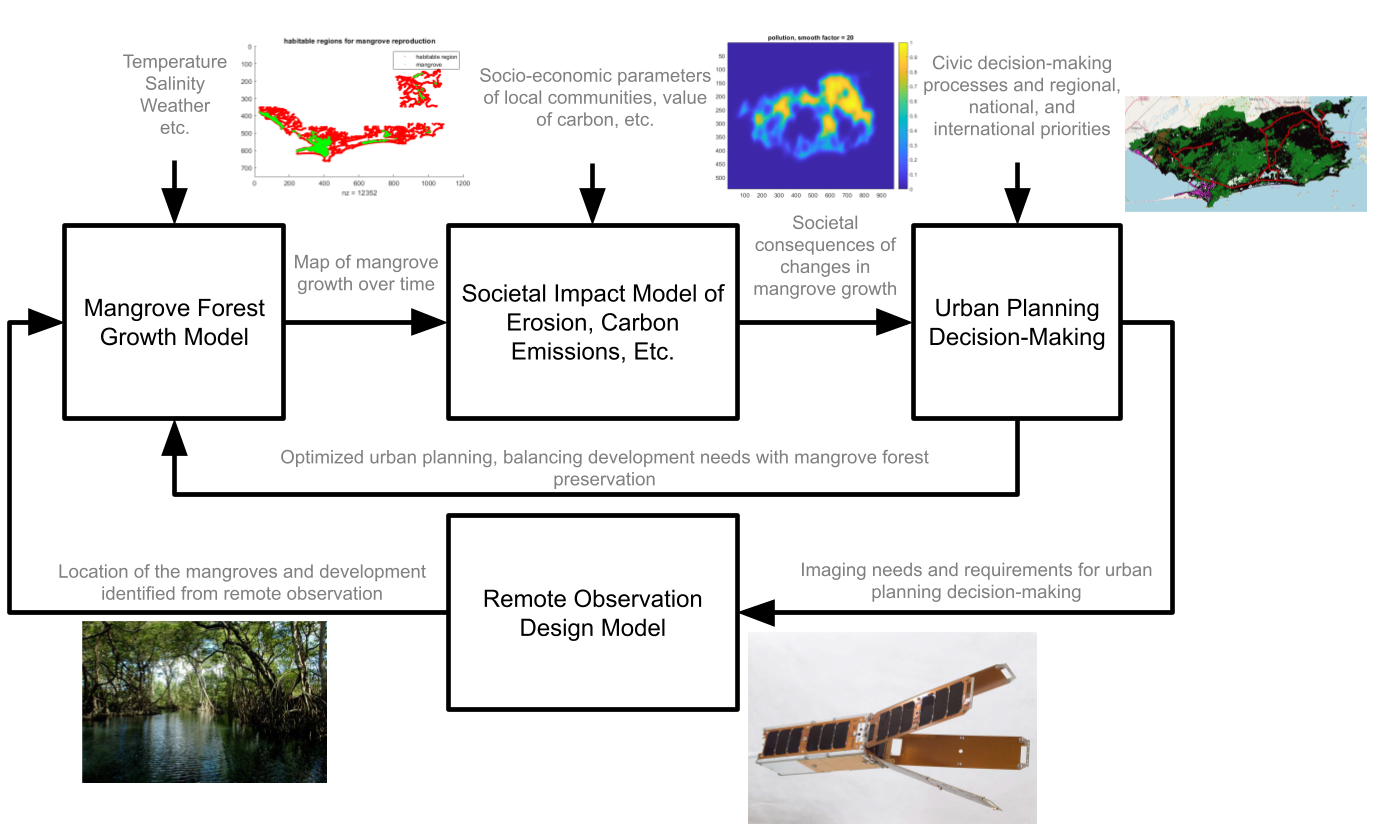
\includegraphics[width=0.9\textwidth]{Figures/chap4/MangroveModelFlow.png}
\caption[EVDT Model (Rio de Janeiro Mangrove Forest Case)]{Environment - Vulnerability - Decision - Technology Model (Rio de Janeiro Mangrove Forest Case)}
\label{fig:rio-evdt-flow}
\end{figure}


\subsection{\hlc[cyan]{EVDT Methodology}} \label{sec:rio-evdt-method}

\subsubsection{\hlc[yellow]{Environment}} \label{sec:rio-evdt-e-method}

The Environment Model of this case study is predominantly interested in the health, the size (as measured by geographic extent), and height of the mangrove forest over time. 

Unlike some other forms of natural resources, which were extensively surveyed and quantified by colonial conquerors and explorers, historical information on pre-industrial Mangrove forest cover tends to be vague, primarily characterizing Mangroves as barriers to settlement \cite{amadorBaiaGuanabaraOcupacao2013}, likely due to historical perceptions of mangroves by colonists, who, as opposed to native inhabitants of the Americas, tended to view mangroves as gloomy sources of disease rather than as natural resources to be exploited \cite{friessEcosystemServicesDisservices2016}. Retroactive understanding of Rio de Janeiro area mangrove cover in this era has been supplemented by palaeoecological studies \cite{vilelaLateHoloceneEvolution2014} but only in a highly incomplete manner. This disregard for mangrove forests largely continued until, after a UN-led effort in the 1980s, international concern over their degradation increased, leading to greater efforts to monitor mangroves. In the second half of the 20th century, mangrove mapping efforts relied primarily on a combination of in-situ surveys and aerial and satellite photography. Investigations were typically site-specific, relied on human interpretation of images, and commonly only had one measurement every 1-2 decades \cite{lacerdaluizandmenezesmarceloandmussimolisanimauricioChangesMangroveExtension2007, fromardHalfCenturyDynamic2004}. These factors limited both spatial scalability and the potential for timely forest management. 
In the past decade, significant progress has been made to address these limitations by creating spatially explicit global mangrove forest cover, loss, drivers of loss, and carbon sequestration maps \cite{spaldingWorldAtlasMangroves2010, donatoMangrovesMostCarbonrich2011, sandermanGlobalMapMangrove2018, simardMangroveCanopyHeight2019, goldbergGlobalDeclinesHuman2020}. Due to both new remote observation datasets and novel analysis techniques,   spatial and temporal accuracy and resolution have significantly increased. The first global mangrove extent map with a consistent methodology and a spatial resolution of <1km was published in 2011 by Giri et al. using data from the Landsat series of \acp{eos} processed by hybrid supervised and unsupervised classification techniques \cite{giriStatusDistributionMangrove2011}. This map represented mangrove forest cover in the year 2000 specifically. More recently, the \ac{gmw} published an extent map with an improved classification methodology covering the years 1996, 2007, 2008, 2009, 2010, 2015, and 2016 \cite{buntingGlobalMangroveWatch2018}. This was accomplished by combining \ac{sar} data from the ALOS PALSAR platform with the Landsat data used by Giri et al. In 2010, the \ac{icesat} with its \ac{glas} was launched. The lidar data generated, when combined with the radar interferometry data from the \ac{srtm} in 2000, has similarly enabled the creation of global mangrove height maps \cite{simardMangroveCanopyHeight2019}, improving carbon storage estimates. Similar advances, often driven by improvements in machine learning, have yielded global maps of human land use, which can be combined with mangrove-related data products to accurately identify drivers of loss \cite{goldbergGlobalDeclinesHuman2020}. Most recently, these tools have been used to generate global datasets in which the specific years of degradation and regrowth are mapped \cite{vancutsemLongterm199020192021}.



\paragraph{\hlc[yellow]{Mangrove Extent}} \label{sec:rio-mangrove-extent} \leavevmode\newline

[** insert diagram of data processing flow, can adapt from one of the conference presentations, see draft in google drive folder]

Regarding extent, the widely-used global mangrove extent maps such as  Giri and\ac{gmw}, are typically representative of specific years and, due to their global-scale, often have higher errors in specific localities, particularly involving the landward edge of mangrove forests and smaller copses of trees. In order to conduct extent-change tracking and to identify such copses, it is sometimes preferred to conduct more targeted estimations, as was done in this case. Mangrove extent was estimated using a Random Forest Classifier (100 trees, 8 variables per split) utilizing both single-band surface reflectance imagery and several multi-band indices from Landsat 7 ETM+, Landsat 8 \ac{oli}, Sentinel 2 MSI, and ALOS PALSAR. Training and validation data was identified using a combination of Giri's 2000 map, \ac{gmw}'s 2015 map, and firsthand field visits. 

[** insert table / figure summarizing training and validation data]

In order to eliminate false positives, a mask was used to filter out flagged pixels at over 40m in elevation, as determined by the \ac{srtm} dataset \cite{jarvisHolefilledSRTMGlobe2008}, and a kernel filter was used to eliminate solitary and near solitary pixels that were erroneously classified as mangroves. This classification, for the year 2018, can be seen in Figure \ref{fig:gextent}. For a more detailed explanation of random forest classifier algorithms and their relevance to forest identification, see \cite{jhonnerieRandomForestClassification2015}.

\begin{figure}[H] 
\centering
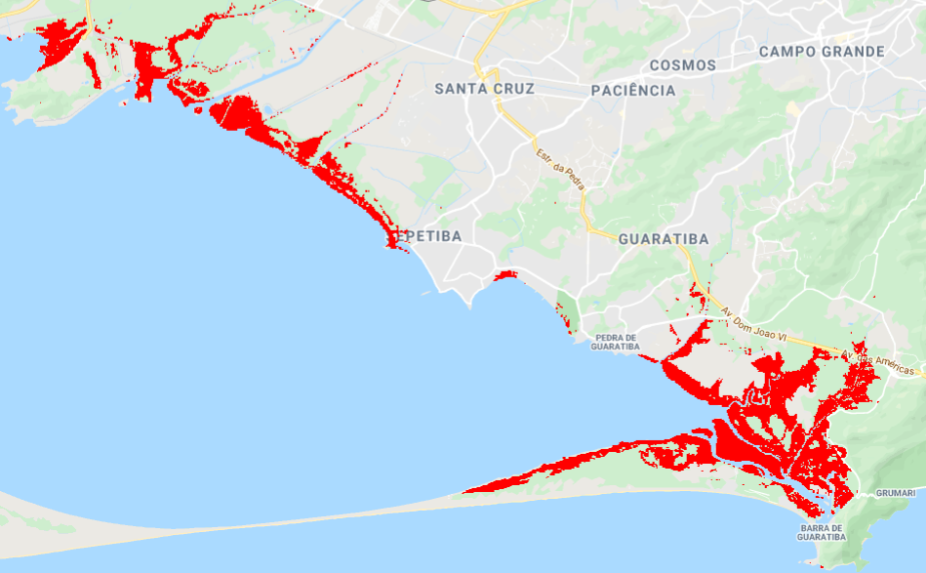
\includegraphics[width=0.49\textwidth]{Figures/chap4/guaratiba_extent.png}
\caption[Classification of mangrove extent in western Rio de Janeiro for the year 2018]{Classification of mangrove extent in western Rio de Janeiro for the year 2018.}
\label{fig:gextent}
\end{figure}

Planet Lab's PlanetScope surface reflectance imagery was also experimented with, but ultimately was determined to not provide sufficient identification improvements to warrant continued use. 

\paragraph{\hlc[yellow]{Mangrove Health}} \label{sec:rio-magrove-health} \leavevmode\newline

The Rio de Janeiro area contains three different species of mangroves (\textit{Avicennia schaueriana}, \textit{Laguncularia racemosa}, \textit{Rhizophora mangle}), each of which have somewhat different spectral reflectance properties, making exact identification and health tracking somewhat more difficult. Ultimately we elected to use the relatively simple and robust \ac{ndvi}, a normalized difference ratio of \ac{nir} and red surface reflectance, as seen in Equation \ref{eq:ndvi}. \ac{ndvi} returns a value between -1 and 1, with 1 indicating a high likelihood of healthy vegetation, -1 indicating an absence of vegetation, and intermediate values indicating either possible vegetation or unhealthy vegetation, as seen in Figure \ref{fig:gndvi}. In Landsat 8's \ac{oli}, the primary instrument used for tracking \ac{ndvi} in this case study, the \ac{nir} band captures \SIrange{0.845}{0.885}{\micro\metre} light while the red band captures \SIrange{0.630}{0.680}{\micro\metre} light. Landsat 5 and 7 surface reflectance imagery were used as well, harmonized according to Roy et al. \cite{royCharacterizationLandsat7Landsat82016}. \ac{ndvi} is the most commonly used surface reflectance index for tracking vegetation presence and health via remote observation, as well as being one of the more commonly used \ac{eo} indices overall \cite{fredenMonitoringVegetationSystems1974,haboudaneHyperspectralVegetationIndices2004, pettorelliUsingSatellitederivedNDVI2005}. 

\begin{equation}
\label{eq:ndvi}
\ac{ndvi} = \frac{NIR - Red}{NIR + Red}
\end{equation}

\begin{figure}[H] 
\centering
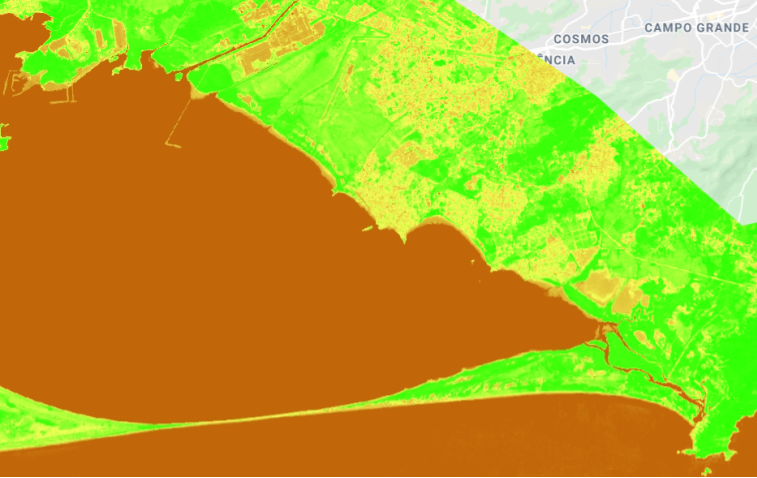
\includegraphics[width=0.49\textwidth]{Figures/chap4/guaratiba_ndvi.png}
\caption[False-Color image of area of interest showing an NDVI composite]{False-Color image of area of interest showing an NDVI composite. The greenest pixels indicate healthy vegetation presence}
\label{fig:gndvi}
\end{figure}

In order to focus on significant, secular changes in mangrove health rather than cyclical or temporary changes, \ac{ndvi} mean anomaly was used, rather than a straightforward \ac{ndvi} time series. The equation for this can be seen in equation \ref{eq:mean}. Here \textit{NDVI\textsubscript{Ref}} refers to the median \ac{ndvi} value at a specific location (an individual pixel in this case) over a specified reference period. \textit{NDVI\textsubscript{i}} refers to the \ac{ndvi} value at that location for each of the images taken during the observation period, and \textit{n} refers to the number of usable images (i.e. clear, no clouds, etc.) at a specific location. As mentioned earlier, \ac{ndvi} is not a perfect measure of mangrove health in a multi-species ecosystem, but it is broadly accurate. With greater number of bands (more than 10) in the visual spectrum, it is sometimes possible to differentiate vegetation species in some cases, but existing free hyperspectral platforms have some combination of poor spatial resolution and insufficient coverage, making them inadequate for this application \cite{mousivandGlobalSensitivityAnalysis2014}. The upcoming launch of the Planet Tanager constellation may alter this situation \cite{planetlabspbcPlanetAnnouncesNew2022}.

\begin{equation}
\label{eq:mean}
Anomaly = \frac{\sum_{i=0}^{n} (NDVI_i - NDVI_{Ref})}{n}
\end{equation}

For this analysis, a reference period of August 31, 1999 to August 31, 2001 and an observation period was September 1, 2001 to September 1, 2018. It should be noted that mean anomaly is sensitive to the selection and duration of these periods, so the presented figures alone should not be taken as indicative of trends outside of the specified periods. 

This \ac{eo} data was accessed and proceed using \ac{gee}, prior to being exported for use as part of the broader \ac{evdt} Modeling Framework. \ac{gee} is a free, cloud-based, geospatial programming platform that hosts free satellite imagery from a variety of sources. This platform obviates the need to download such imagery onto a computer for individual manual analysis. This method of extent and health tracking is largely based upon methods used by Lagomasino et al. \cite{zhangModelingRiskMangroves2019}. Once this historical mangrove data has been processed, it serves as the foundation of estimating causal impacts between the \ac{evdt} components.

\begin{figure}[H] 
\centering
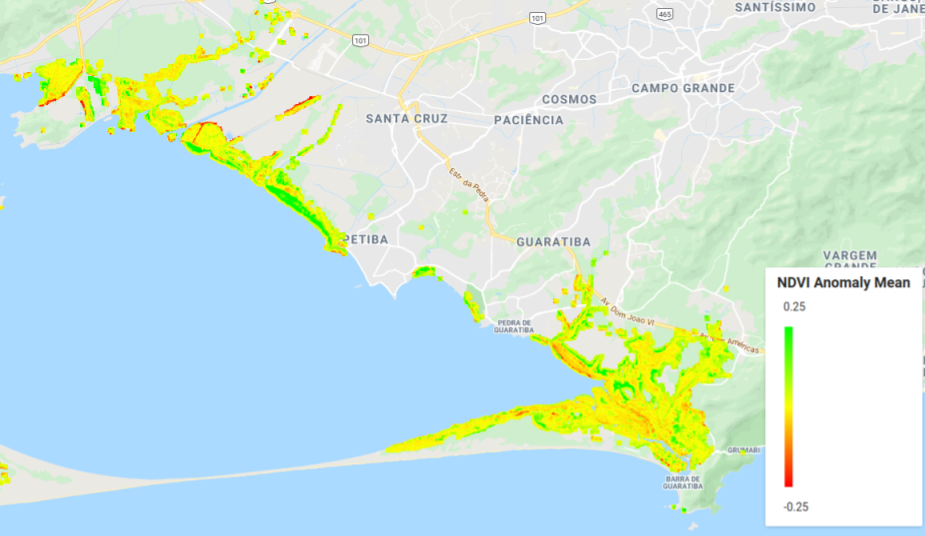
\includegraphics[width=0.49\textwidth]{Figures/chap4/guaratiba_anomaly.png}
\caption[False-Color image depicting NDVI mean anomaly]{False-Color image depicting NDVI mean anomaly. Green indicates new or healthier mangroves, red indicates reduction in extent or in health, yellow indicates no measured change.}
\label{fig:anomaly}
\end{figure}

\paragraph{\hlc[yellow]{Mangrove Height}} \label{sec:rio-mangrove-height} \leavevmode\newline

More specifically to the Rio de Janeiro area, height of mangrove trees can be measured using aerial \ac{lidar} \cite{olagokeIndividualMangroveTree2015} and Rio de Janeiro has recently conducted such a survey of the entire municipality, though the data was not available in time for this work. Once it is, the height can be used to estimate \ac{agb} \cite{cloughAllometricRelationshipsEstimating1989, fatoyinboEstimatingMangroveAboveground2018}, which is important for improving estimates of the forests' carbon sequestration capabilities \cite{lagomasinoMeasuringMangroveCarbon2019}. Historical height data can be estimated using space-based \ac{lidar} and \ac{sar} data \cite{lagomasinoComparisonMangroveCanopy2016}, though this method lacks the spatial resolution of aerial methods.

[** add more text and figures about the height statistics in this region specifically]

\subsubsection{\hlc[yellow]{Vulnerability}} \label{sec:rio-vulnerability}

[** summarize the datasets and outputs discussed in this section in a table]

Social impact and vulnerability in this case study has several different forms. First there are general socioeconomic trends and pressures in the Guaratiba area. A qualitative history of these was presented in Section \ref{sec:rio-context}. In addition to this history, various quantitative socioeconomic and demographic data, including employment rates and population density, were collected at several geographic scales, including bairros (neighborhoods), census blocks, and census microgrids. Much of this data was sourced from the national statistics agency, the \ac{ibge}. These were supplemented with municipally collected data, organized by \ac{ipp}. Such data includes a UN-developed \ac{ipm} \cite{oxfordpovertyandhumandevelopmentinitiativeChartingPathewaysOut2020}, a municipally-customized social progress index \cite{puliciRelatorioMetodologicoIndice2016}, and detailed land use / land cover maps \cite{regoAutomaticClassificationLand2003}. This data varies significantly in its geographic and temporal resolution. 

The second form of social impact and vulnerability comes in the form of ecosystem services provided, directly or directly, by the mangroves. Ecosystem services are often sorted into three categories: provisioning (providing some raw material), regulating (moderating the ambient environment in a helpful manner), and cultural (non-material benefits) \cite{haines-youngCommonInternationalClassification2018}. Mangrove forests around the world provide each of these:

\begin{itemize}[itemsep=0pt,parsep=0pt]
	\item{Provisioning: Fuelwood / timber}
	\item{Regulating: Water filtration, protection from coastal erosion and storms\footnote{Some studies place protection from coastal erosion and storms into a fourth category, supporting/maintaining, rather than in regulating \cite{getznerEcosystemServicesMangrove2020}.}, hosting fisheries}
	\item{Cultural: Tourism, general biodiversity}
\end{itemize}

As mentioned previously, it is known that the local communities in the Guaratiba area benefit from various ecosystem services provided by the mangroves, but the exact forms these services take are unknown and their values have not been quantified. Some bounds on these values can be estimated from valuation studies focusing on mangroves elsewhere in the region and elsewhere around the world. To this end, we examined mangrove ecosystem services valuations from the \ac{esvd} \cite{grootEcosystemServicesValuation2020} (an open source database maintained by the Foundation for Sustainable Development) and nine meta-analyses or review papers \cite{branderEmpiricsWetlandValuation2006,branderEcosystemServiceValues2012, salemEconomicValueMangroves2012, veghMangroveEcosystemServices2014, voReviewValuationMethods2012, himes-cornellMangroveEcosystemService2018, getznerEcosystemServicesMangrove2020, barbierProtectiveServiceMangrove2016, barbierEstuarineCoastalEcosystems2020} in order to determine a potential range of values for the various mangrove ecosystem services in the Guaratiba area. Additionally, we use Simard et al.'s global map of mangrove canopy height, \ac{agb}, and carbon stock per hectare in the year 2000 \cite{simardMangroveCanopyHeight2019} to provide a baseline carbon storage estimate for the Guaratiba mangroves. We can use changes in mangrove extent over the 2000-2018 period to estimate likely changes in carbon stocks. In the future, when the aforementioned aerial \ac{lidar} survey data becomes available, these estimates can be revised.


\subsubsection{\hlc[cyan]{Decision-making}}

Two primary policy decisions are currently included in this \ac{evdt} application: conservation status and urban zoning. The histories of these are provided by the municipal Environmental Secretariat and Urban Planning Secretariat and accessed via the Data.Rio platform. The urban zoning categories are broadly similar to those in many cities around the world and include the types of commercial and industrial activity permitted and maximum floor area ratio allowed, among other factors. 

Conservation status, on the other hand, is more complicated, as discussed in Section \ref{sec:rio-jurisdictions}. Some of these protected areas are classed as ``integral protection," meaning little or no development and resource extraction is allowed. In addition to these areas (and often surrounding them), there are various municipally-defined ``sustainable use" areas that allow for certain, restricted forms of development and resource extraction. There are also two different classes of ``boundary zones" with yet fewer protections.

In addition to conservation, there is the potential for replanting and restoration of mangroves. Numerous replanting and restoration projects have taken place in the Rio de Janeiro area in recent years, both in dedicated conservation areas \cite{granadoAssessingGeneticDiversity2018} and in more urban and peri-urban areas \cite{rioprefeituraEnvironmentalRecoveryRodrigo2019, soaresEstruturaVegetalGrau1999}. Siting of these restoration areas ideally depends both on the environmental viability of a potential site and its likely ecosystem service impacts.

The selection of these two axes of policy decisions (conservation status and urban zoning) was based on meetings and discussions with government officials from several municipal and federal agencies, university researchers, and local community members. Other axes were discussed and were of interest to particular audiences (such as transit network changes and conservation policy enforcement stringency), but these two held broad appeal and relative accessibility, while still having concrete historical data that are either quantitative or code-able qualitative in nature. 



\subsubsection{\hlc[red]{Technology}}

[will look at the history of remote sensing use in Rio de Janeiro]

[consider possible additional sensing uses/platforms in the future]

[discuss options future steps beyond the scope of this thesis (tradespace exploration)?]

\subsection{\hlc[red]{EVDT Results}} \label{sec:rio-evdt-result}

\subsubsection{\hlc[yellow]{Environment}} \label{sec:rio-evdt-e-result}

[quantitative changes in mangrove extent]

[compare changes in protected areas to changes outside of protected areas]

[discuss areas of particularly notable gain or loss, tie into other developments]
	[steel mill construction]
	[highway and rapid transit line]
	[potential wood beetle infestation]

\subsubsection{\hlc[yellow]{Vulnerability}} 

[quantitative socioeconomic/demographic data from IBGE census and multidimensional poverty index]

[estimates of mangrove ecosystem services from review of valuation studies]

[calculation of year 2000 carbon stock, then how changes in extent could have impacted that]

\subsubsection{\hlc[yellow]{Decision-making}} 

[revisit how mangroves fared inside and outside of protected areas]

[discuss enforcement, including differential enforcement]

[fishers want control over where mangrove replanting occurs]

[consider moving the recommendations synthesized from previous reports in the System Context section here]

\subsubsection{\hlc[yellow]{Technology}} 

The city of Rio de Janeiro has made significant use of \ac{eo} data dating back to 1975, as can be seen in Table \ref{tab:history}, but it is only in recent years that this data usage has become fairly regular. Even now, there has not been any particular consistency with the choice of imagery source, with the city switching back and forth between aerial and satellite surveys every few years. And there has been a significant lack in the use of civil scientific satellites such as Landsat for mapping and decision-making purposes, further pointing towards the need for tools to facilitate the use of such satellite data.

\begin{table}[H]\centering
	\caption[EO data use by Rio de Janeiro]{\ac{eo} data use by the  municipal Urban Planning Secretariat of Rio de Janeiro}\label{tab:history}
	% \small
	\fontsize{8}{10}\selectfont
	\csvreader[tabular=|C{0.8cm}|L{4cm}|L{5cm}|, 
		table head=\hline 
		\textbf{Year} & \textbf{Product} & \textbf{Platform} \\ \hline,
		table foot=\hline,
		late after line=\\\hline]
		{Figures/chap4/eo_history.csv}%
		{1=\year,2=\type,3=\platform}
		{\year & \type & \platform}
\end{table}

[research and mapping programs by espaco and others]

\section{\hlc[red]{Decision Support System}} \label{sec:rio-dss}

\subsection{\hlc[red]{DSS Methodology}}

[explain process and software used for the DSS]

\subsection{\hlc[red]{DSS Results}}

[explain the state of the prototype]

[insert screenshots]

[insert link to code]

\begin{figure}[t] 
\centering
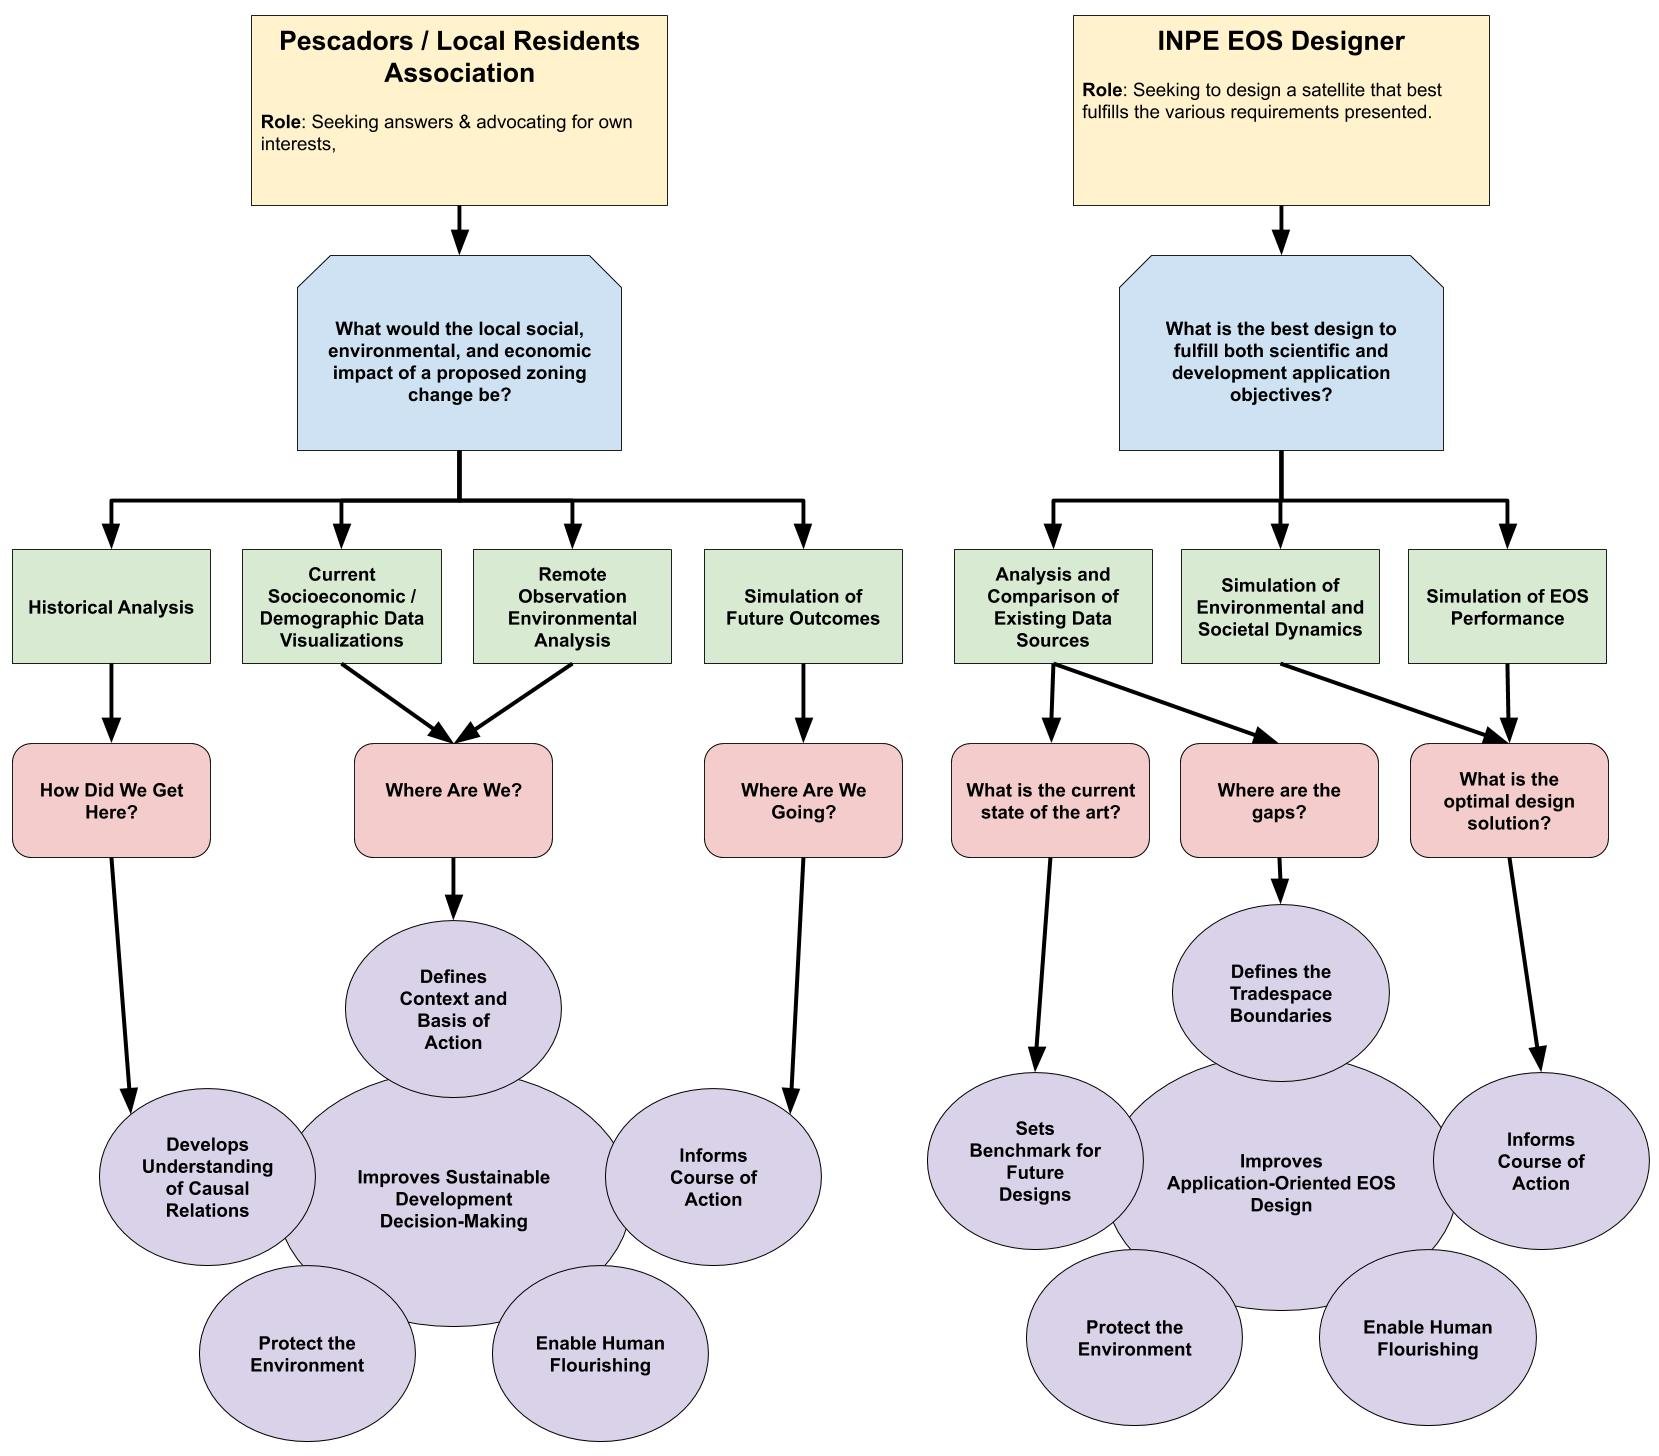
\includegraphics[width=0.9\textwidth]{Figures/chap4/concept_flow.jpg}
\caption[Two potential user experience concepts for the Rio de Janeiro case study]{Two potential user experience concepts for this case study}
\label{fig:concept_flow}
\end{figure}

\section{\hlc[red]{Collaborative Development Process}} \label{sec:rio-collab}


[discuss ongoing collaboration beyond the initial interviews]


\section{\hlc[red]{Discussion}} \label{sec:rio-discussion}


evidence that the protected areas in the greater Rio de Janeiro have helped the mangroves \cite{cavalcantiEvaluatingMangroveConservation2009}

replanting mangroves helps the soil \cite{jimenezRecoverySoilProcesses2022}

[lessons learned]
	[pros and cons of having a fairly neutral (at least as far as the government is concerned) primary point of contact]
	
[potential for future development]
	[moving online]
	[informing the bounds of APA da Orla da Baía de Sepetiba]
	[household survey studies to inform ecosystem services]
	[use aerial lidar survey to revise height / biomass estimates]
	[use of Planet Tanager for species differentiation]

Beyond the scope of this thesis, in order to better understand and quantify the dynamics linking mangrove health and conservation policies with local socioeconomic impact, the team is currently pursuing collaborating with an ecosystem services economist to analyze historical data and potentially to conduct household surveys. This historical data will be used in conjunction with the mangrove health history to estimate the "Carbon and Raw Material Impact" and "Local Socioeconomic Impact of Mangrove Loss," as shown in Figure \ref{fig:method}. For more details on these types of methods, see \cite{jungBrazilNationalEnvironmental2017, jungPartnershipsPreventDeforestation2018}. Once these historical dynamics are better understood, we can progress to predictive simulation of vulnerability.


\begin{figure}[t] 
\centering
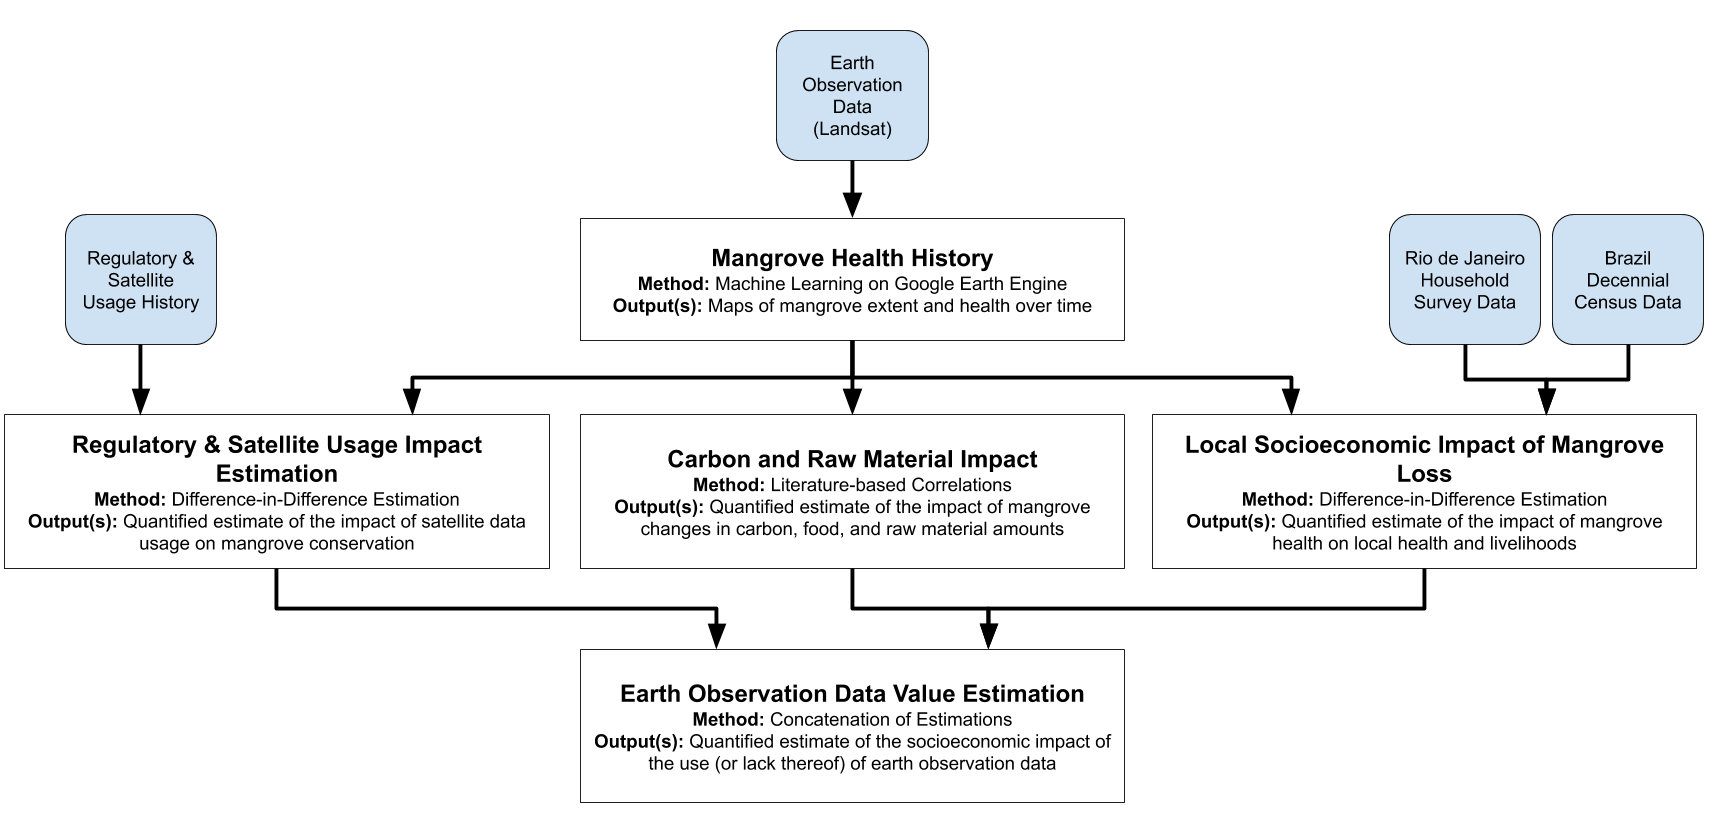
\includegraphics[width=0.9\textwidth]{Figures/chap4/Method_Flowchart.png}
\caption{Flowchart indicated various ways of estimating causal impact of one EVDT component on another}
\label{fig:method}
\end{figure}

The history of these two policy axes over the past several decades will be used in conjunction with the Environment and Vulnerability Models to estimate the regulatory impact on these two domains, as shown in Figure \ref{fig:method}.

\section{\hlc[red]{Conclusion}}






